\section{Zed Attack Proxy}
\frame{
	\frametitle{Zed Attack Proxy}
	\framesubtitle{Basics}
	
	\begin{itemize}
		\item Open-source web scanner by the Open Web Application Security Project
		\item Used as the basis for the demo later
	\end{itemize}
}

\frame{
	\frametitle{Zed Attack Proxy}
	\framesubtitle{Basics}
	
	\begin{figure}
		\centering
		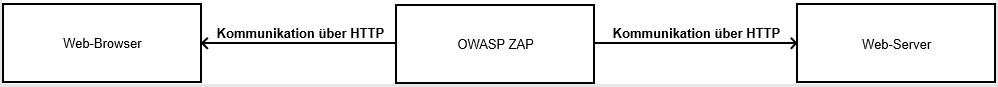
\includegraphics[width=1.0\linewidth, height=0.3\textheight]{content/img/MIM}
		\caption{ZAP used as a Man-in-the-middle Proxy}
		\label{fig:mim}
	\end{figure}
	
}

\frame{
	\frametitle{Zed Attack Proxy}
	\framesubtitle{Usage}
	
	\begin{itemize}
		\item Automatically finding of vulnerabilities in applications
		\item Allows developers to integrate pentesting and security regression in a CI/CD pipeline
	\end{itemize}
}